\chapter{Evaluation}
\chaptermark{Evaluation}
\addcontentsline{toc}{chapter}{Evaluation}  

Preprocessing time, space consumption of the precomputed auxiliary data, query processing time and space, the ability for multi-criteria optimization (travel times, number of transfers, prices, etc.), realistic modelling (transfer buffers, footpaths), and the ability to deal with delays and other real-time information.
\section{MongoDB Storage}
We created a merged view for our entry point. The connected entities are embedded in our scheduled stop point. This ensures we can quickly look up each station using \glsxtrshort{raptor}.

However, we also added the rest of the information to separate collections of MongoDB. This ensures we can look up information after route planning. You can get either the entity alone or an entity and all its referenced entities. They are returned as a graph and are not embedded. The code for resolving all the references in an entity can be found in \autoref{code:resolve}. An example can be found in \autoref{code:example:line}.

\begin{table}[H]
\centering
\begin{tabular}{|l|l|l|l|l|l|}
\hline
\textbf{} &
  \textbf{\begin{tabular}[c]{@{}l@{}}Number of\\  documents\end{tabular}} &
  \textbf{\begin{tabular}[c]{@{}l@{}}Avg. \\ document size\end{tabular}} &
  \textbf{\begin{tabular}[c]{@{}l@{}}Number \\ of indexes\end{tabular}} &
  \textbf{\begin{tabular}[c]{@{}l@{}}Total\\  index size\end{tabular}} &
  \textbf{\begin{tabular}[c]{@{}l@{}}Total\\ storage size\end{tabular}} \\ \hline
AutoriteitOfOperator   & 1    & 134B     & 1 & 20.48kB  & 20.48kB  \\ \hline
Dienstkalender         & 9.7K & 24.71kB  & 1 & 151kB    & 151.57MB \\ \hline
Dienstrit              & 37K  & 309B     & 1 & 831.49kB & 2.05MB   \\ \hline
Dienstritpatroon       & 37K  & 2.27kB   & 1 & 811.01kB & 10.83MB  \\ \hline
Doorkomsttijd          & 652K & 216B     & 1 & 9.22MB   & 15.26MB  \\ \hline
Lijn                   & 856  & 479B     & 1 & 28.67kB  & 73.73kB  \\ \hline
Merged                 & 2.6K & 301.22kB & 5 & 31.07MB  & 67.70MB  \\ \hline
Route                  & 856  & 4.82kB   & 1 & 28.67kB  & 733.18kB \\ \hline
Stopplaats             & 2.6K & 209B     & 1 & 7373kB   & 98.30kB  \\ \hline
StopplaatsInRitpatroon & 652K & 715B     & 2 & 17.79MB  & 45.39MB  \\ \hline
\end{tabular}
\caption{Statistics in MongoDB of our result.}
\label{tab:mongodbstatres}
\end{table}
We can see that indexing is using a lot of storage. The problem is indexes on embedded documents, which are necessary to speed up our creation time.
% todo add implementation in appendix
\subsection{comformity of ontology}
\subsubsection{comformity application profiles}
\glsxtrshort{oslo} has also described when a \glsxtrshort{jsonld} document conforms to an application profile \cite{noauthor_conformiteit_nodate}.

An application profile is a specification for data exchange that introduces additional constraints for applying vocabularia. These constraints could include refinement of terminology (classes and properties) consistent with the semantics from the relevant specifications with a well-defined usage as a goal;
    External terminology (classes and properties) is used for new/extra terms not found in the existing vocabulary.

To conform with the \glsxtrshort{oslo} application profile, the following constraints have to be met:
\begin{itemize}
    \item \textbf{Must} each class contains the attributes that have a cardinality of one/
    \item \textbf{Forbidden} for a class attribute with a cardinality of maximum one to have more instantiations.
    \item \textbf{Forbidden} to use terminology of vocabularia not defined in the application profile.
    \item \textbf{Allowed} to use terminology in a way that is consistent with her semantics (definition, use, domain and range)
    \item \textbf{Allowed} to extend with other vocabularies that do \textbf{do not overlap} with terminology from this vocabulary. 
\end{itemize}
\subsubsection{\glsfmtfull{shacl}}

The \glsxtrshort{oslo} organisation also provides a shacl file that describes the ontology constraints. This also includes cardinality.

We tested our merged Scheduled Stop Points. First, we took one scheduled Stop point and added our context file. Then proceeded to transform the \glsxtrshort{jsonld} document to N-Quads using @rdfjs/parser-jsonld \cite{noauthor_rdfjs-baseparser-jsonld_2024}. We then read the Shacl File and provide both turtle files to the \glsxtrshort{shacl} validator \cite{noauthor_rdf-validate-shacl_2024}.

We got good results back, THe main constraint was a ClassConstraint violation. Mainly, this was caused by the fact that the entity that a \glsxtrshort{iri} was pointing to was not in the graph.

\section{Fragmentation evaluation}
We wrote a quick Python script for a first but straightforward evaluation of our fragment strategies. The duration (\autoref{fig:fragduration}) is the total duration to make a request, receive the request and do some processing from the client's viewpoint. The size (\autoref{fig:fragsize}) is the total size of a request, including headers.

For these measurements, a list of 100 stations was randomly selected out of all possible stations. For this, we used $random.choice()$. When a destination station was needed, we selected another 100 stations. Then, we made our requests to the server.

\begin{figure}[H]
    \centering
    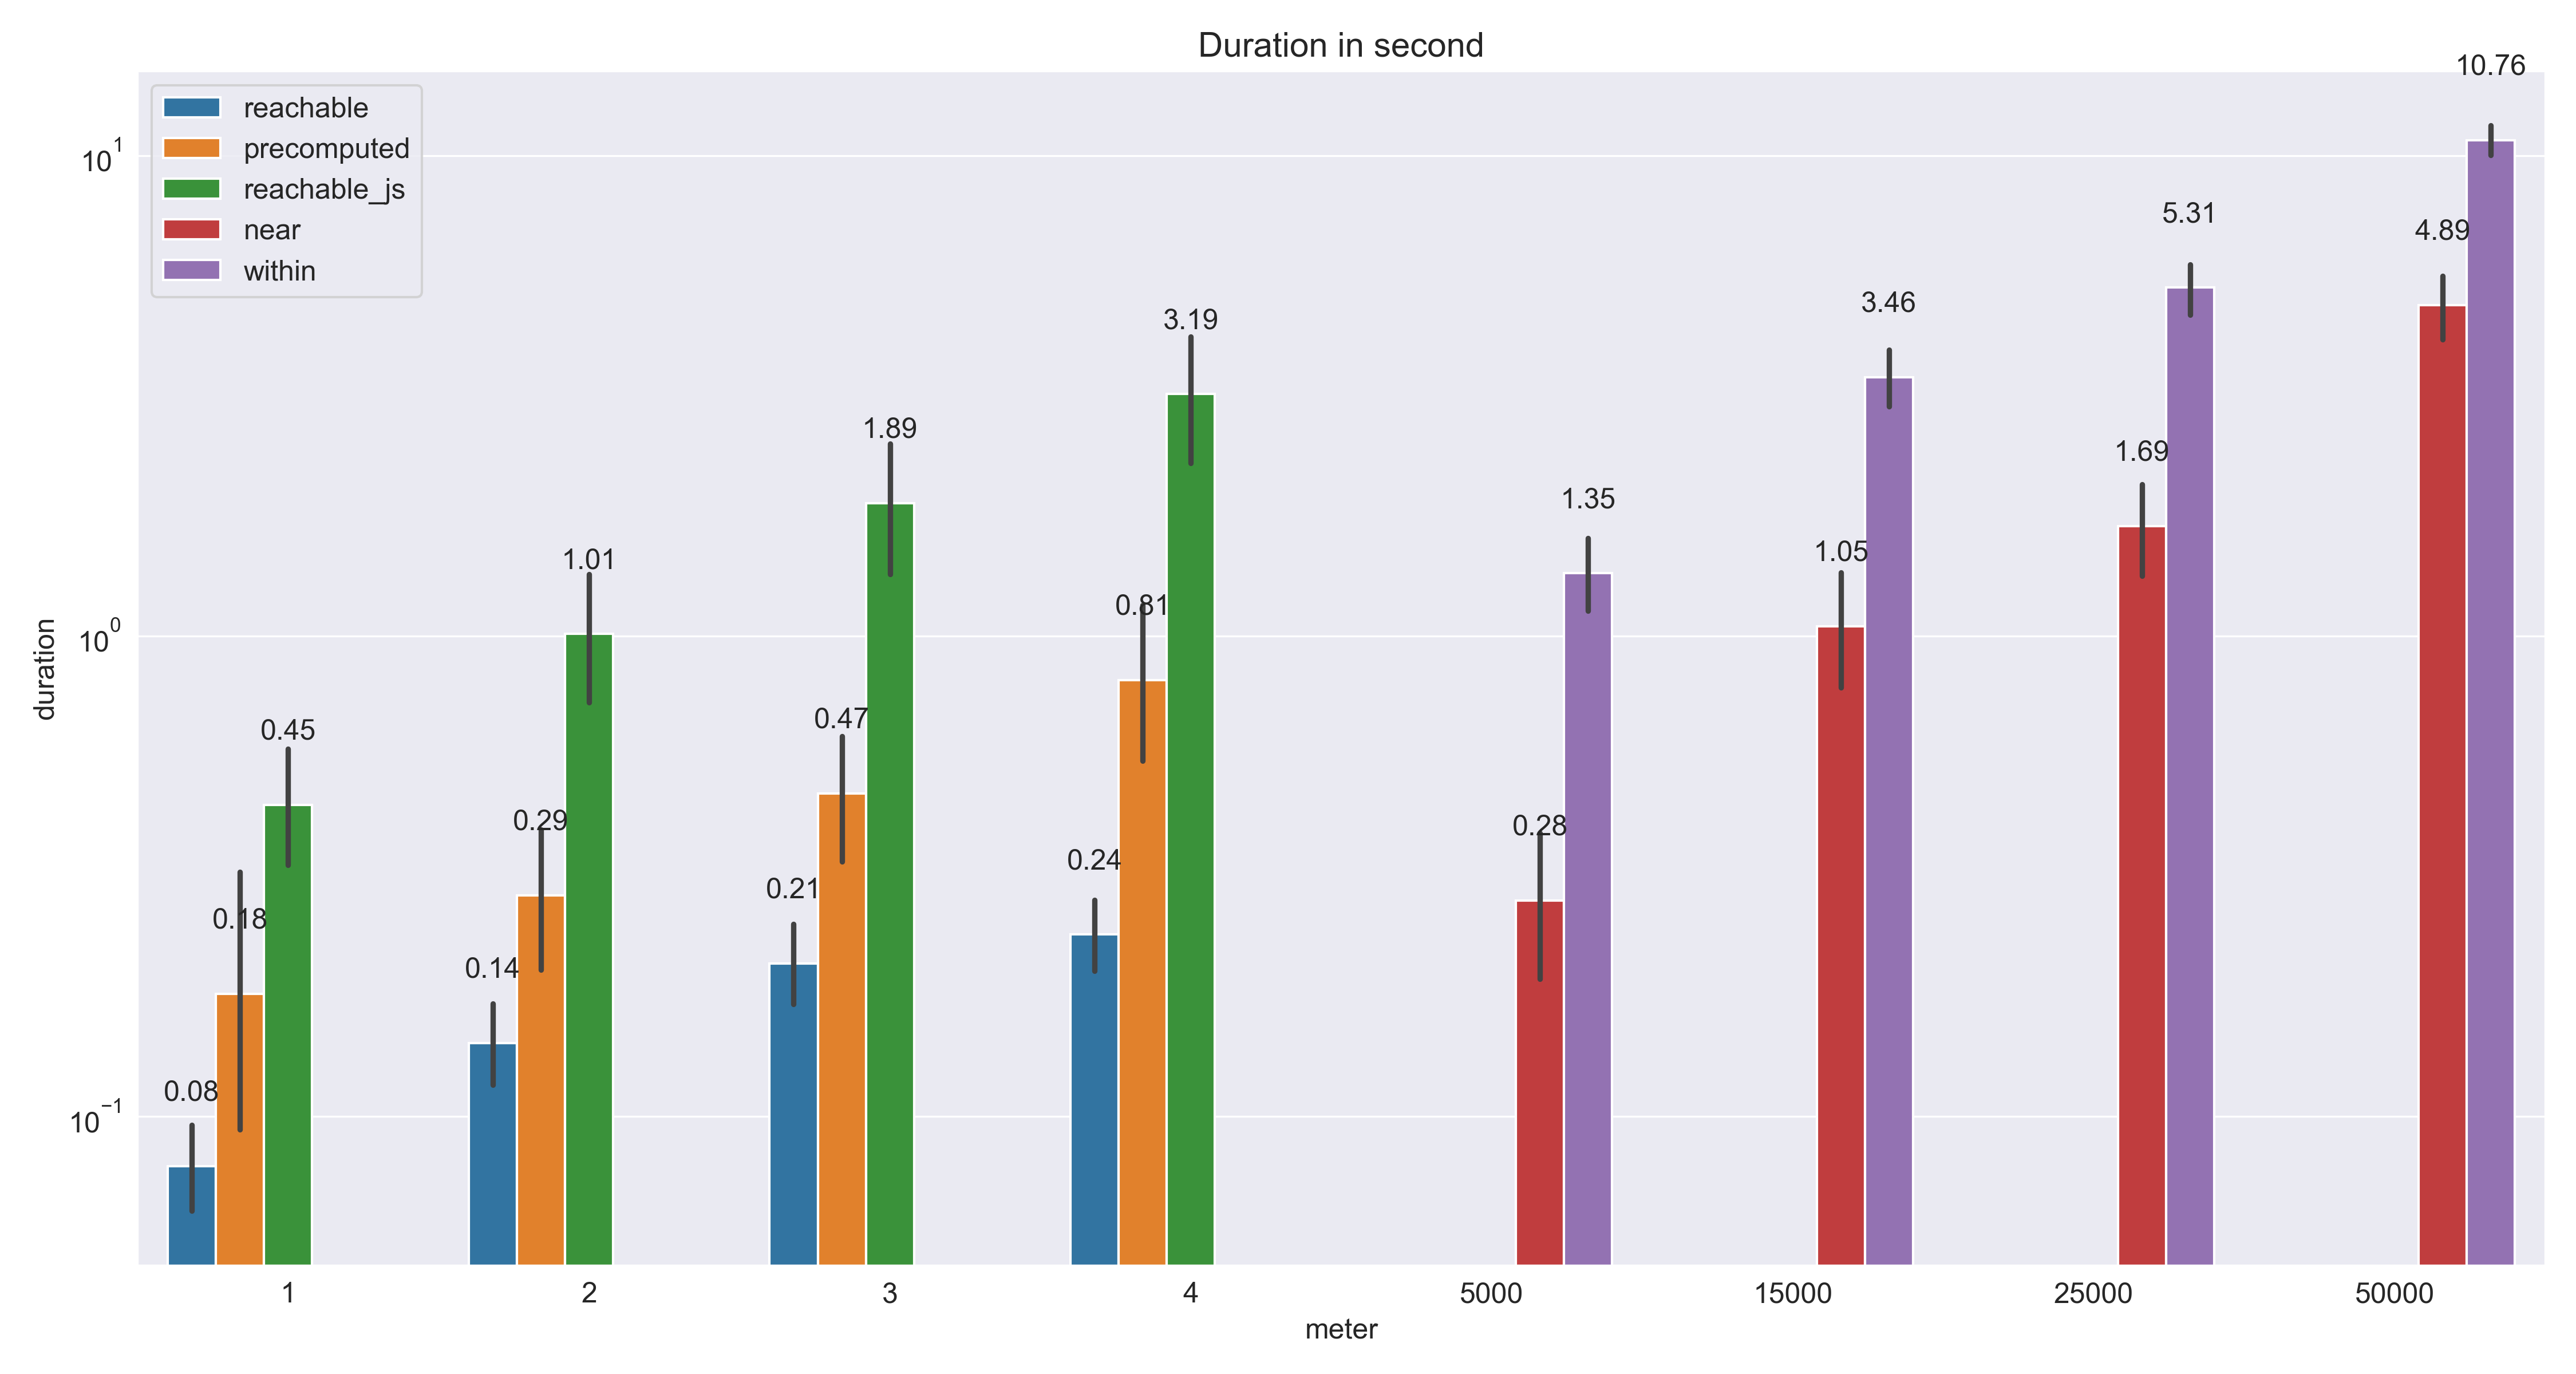
\includegraphics[width=\textwidth]{images/fragmentsbyduration.png}
    \caption{Some tests measure the response time and processing time needed to receive a fragment. The left four on the x-axis use a k as a parameter, and the right four use meters as a parameter. The Y-axis is in the log scale!}
    \label{fig:fragduration}
\end{figure}
\begin{figure}[H]
    \centering
    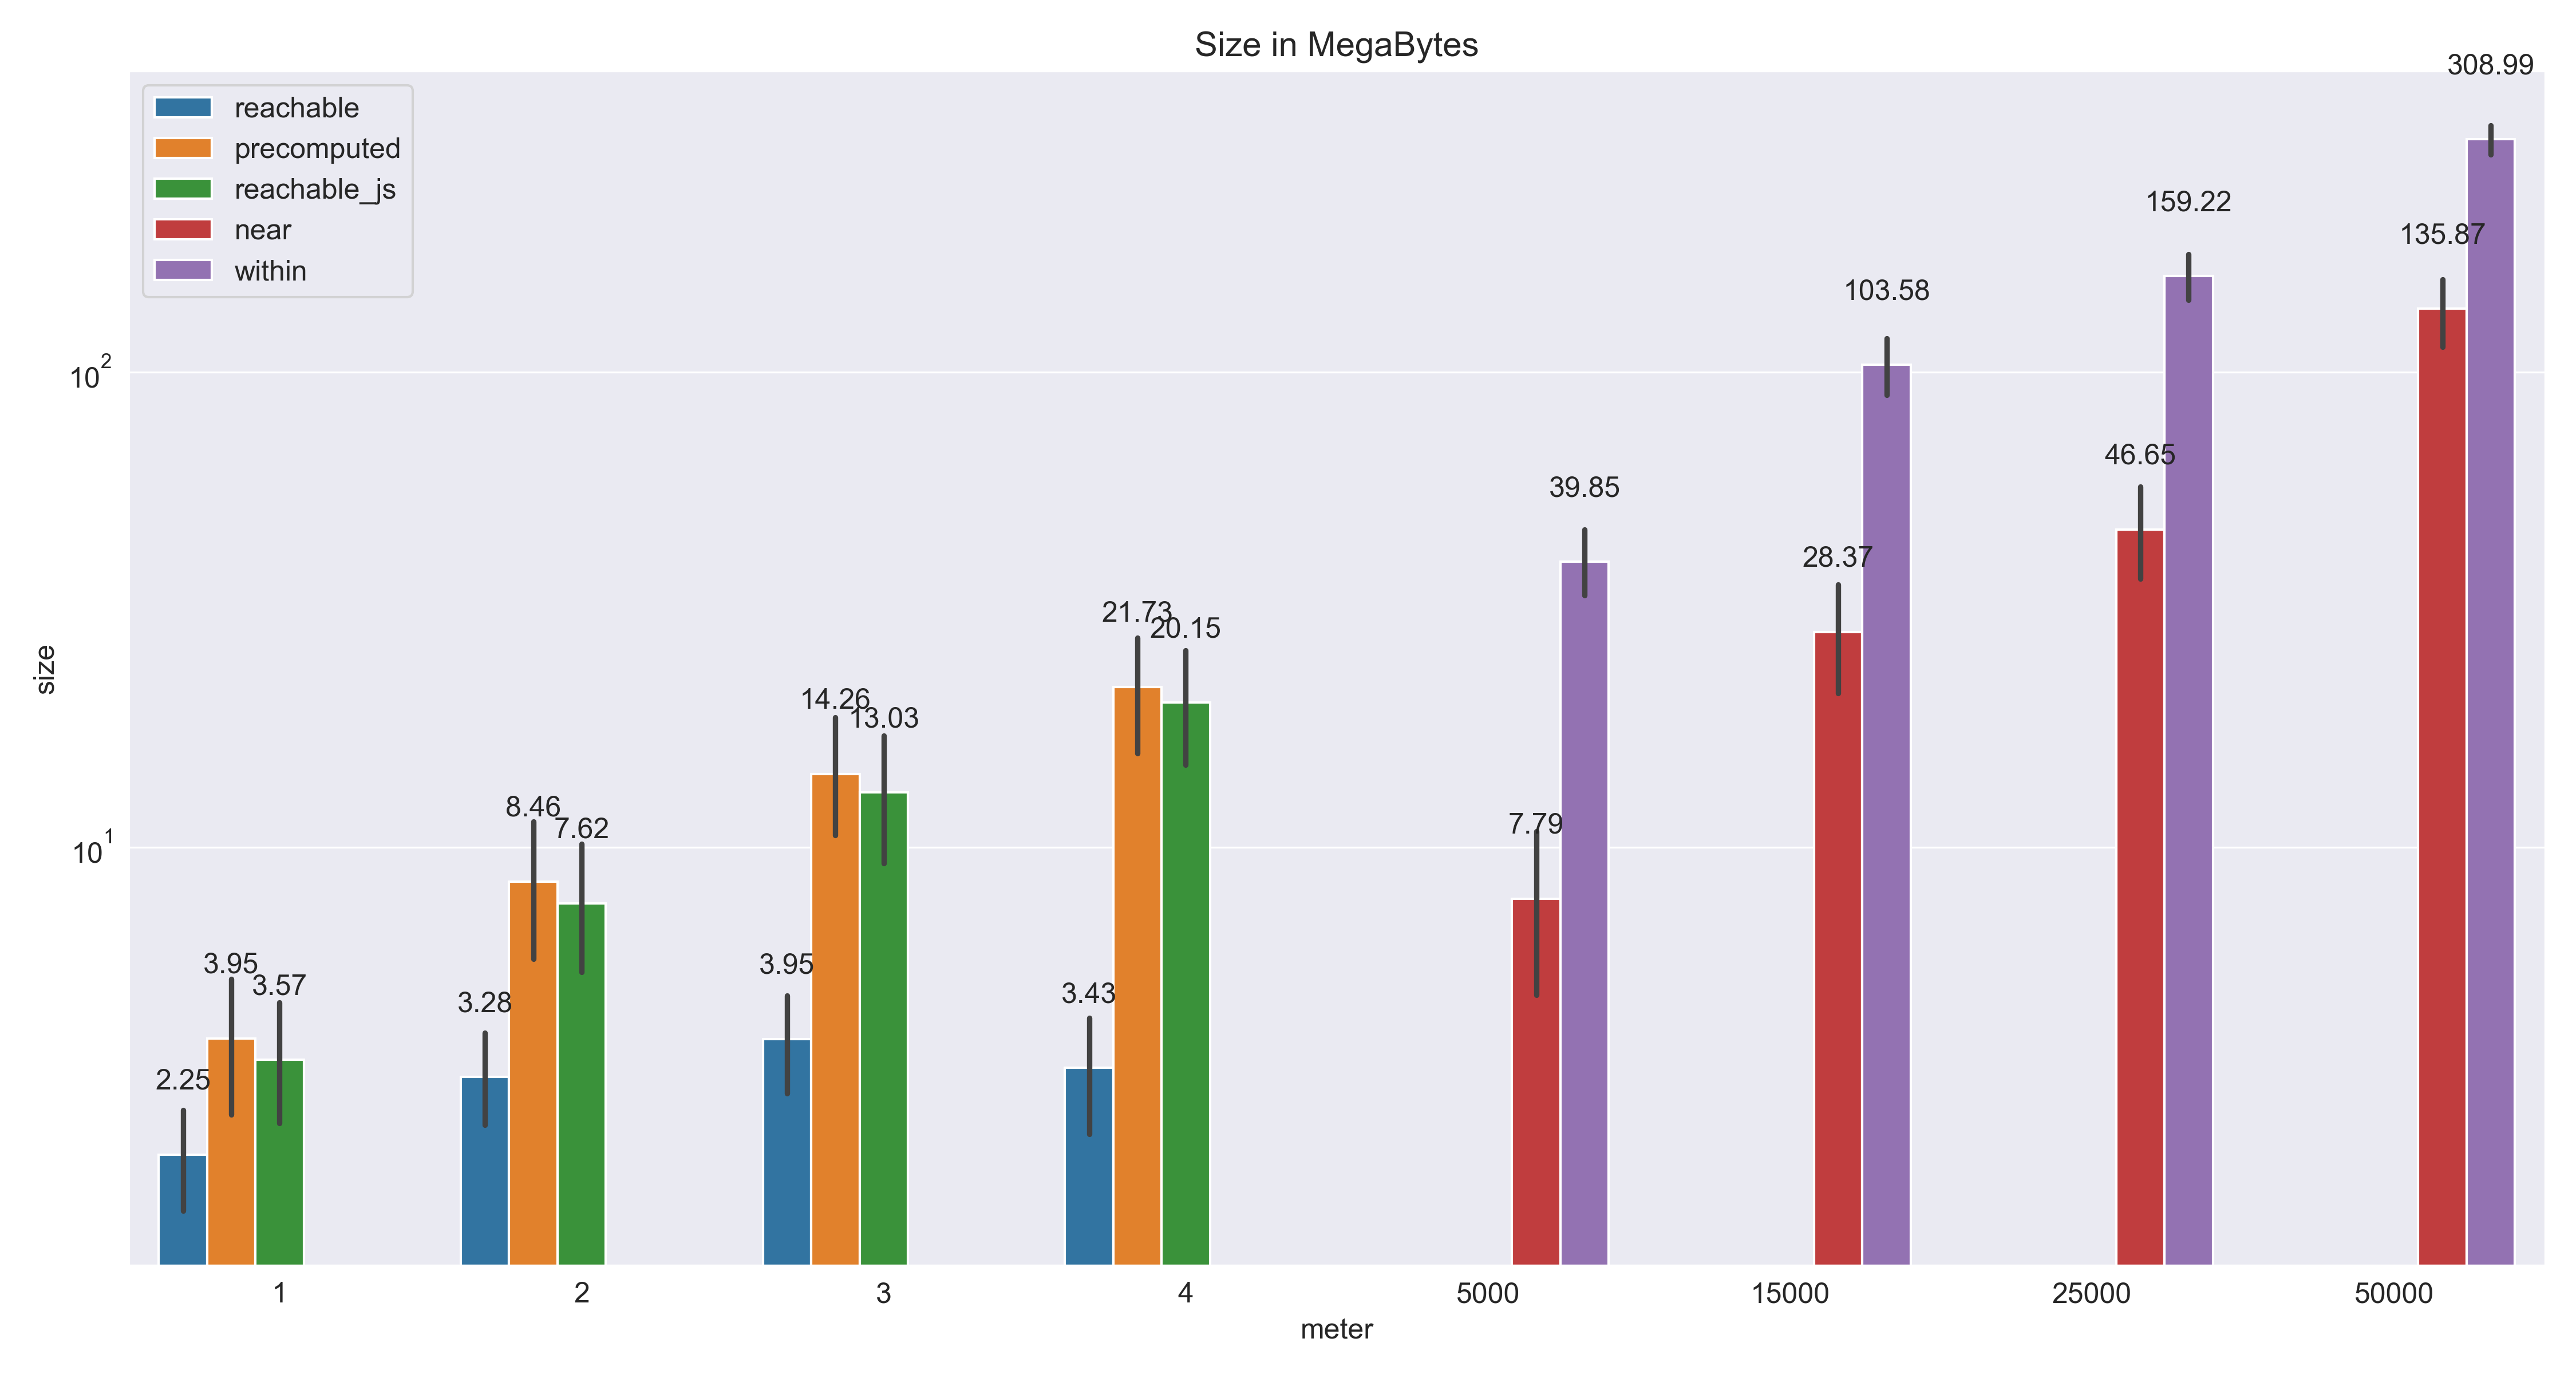
\includegraphics[width=\textwidth]{images/fragmentsbysize.png}
    \caption{Some tests to measure the size of a fragment. The left four on the x-axis use a k as a parameter, and the right four use meters as a parameter. The Y-axis is in the log scale!}
    \label{fig:fragsize}
\end{figure}


If we look at \autoref{fig:fragduration}, we see that the reachable strategy is the fastest. The JavaScript version quickly becomes slower with higher k values. The precomputed version indeed saves time compared to the javascript version. 

The reachable implementation using $\$graphLookup$ is the fastest, but we can not trust the graph as K grows. As graphlookup errors, when passing the 16 Megabyte limit, it can only handle the subset of selected stations without many connections. 

The near strategy is pretty fast, but it has trouble finding any relevant stations for small values. We must use a significant parameter for long-distance travel, selecting even more irrelevant stations. 

The within strategy is generally relatively slow and has the most size. This is logical since it typically spans a large area and, depending on the buffer size contains many stations. This is probably the leading cause of its slowness. This can be seen as an advantage and a weakness. It presumably includes a lot of relevant stations; since the chance is very high, we have to pass by a station between our source and destination stations. But presumably, it also contains a lot of stations we do not pass by. We still have fewer irrelevant stations than using the near strategy. 